\label{soluzione_problematiche}
\subsection{Entit\`{a} Circuito}
\label{entita_circuito}
Nella soluzione proposta il circuito è un'unità composta da più entità passive
ad accesso mutuamente esclusivo. Più precisamente:
\begin{itemize}
\item \textbf{Path}: rappresenta la traiettoria percorsa da un concorrente. Un
insieme di \textbf{Path} costituisce un tratto e il loro
numero all'interno del tratto identifica la molteplicità dello stesso. Ogni path
è caratterizzato da:
\begin{itemize}
\item lunghezza
\item angolo
\item tenuta
\item istante di liberazione
\end{itemize}
I \textbf{Path} di uno stesso tratto possono essere uguali o differire per
caratteristiche, rimanendo comunque entro i limiti globali del tratto
(non si potrà ad esempio avere un tratto lungo 11 km in un tratto lungo 42 m).\\
Per quanto riguarda l'\textbf{istante di liberazione}, esso indica da che
istante non ci saranno più concorrenti sul \textbf{Path}.
\item \textbf{Checkpoint}: è una risorsa passiva ad accesso mutuamente
esclusivo. Rappresenta la coda di accesso ad un tratto. Ogni posizione
della coda è stata arricchita con delle informazioni che aiutano a gestire
l'accesso al tratto:
\begin{itemize}
\item \textbf{istante di arrivo}: l'istante di tempo più ottimista in cui l'auto
è prevista arrivare oppure l'istante in cui l'auto realmente
arriva al tratto (in base al valore della flag ``arrivato'', descritta in
seguito);
\item \textbf{id concorrente}: l'id del concorrente presente nella posizione
della coda;
\item \textbf{flag ``arrivato''}: se valorizzata con \emph{true}, significa che
il concorrente sta effettivamente attendendo di accedere al tratto
e che il valore temporale segnato nell'\textbf{istante di arrivo} è l'istante di
arrivo effettivo. Altrimenti significa che il concorrente non
è ancora arrivato ma arriverà ad un istante maggiore o uguale a quello segnato
nell'\textbf{istante di arrivo}.
\end{itemize}
Ogni \textbf{Checkpoint} inoltre punta ad un insieme di \textbf{Path}.
\item \textbf{Racetrack iterator}: ogni concorrente dispone di un'istanza di
questo iteratore per poter navigare il circuito e richiedere
di accedere eventualmente ai box.
\end{itemize}
La struttura è stata pensata principalmente per venire a capo del problema dei
sorpassi impossibili.\\
Come visto nella sezione \ref{tempo}, non esiste un orologio assoluto. Ogni
concorrente segna sulla
coda il tempo di arrivo in base ai tempi accumulati per l'attraversamento dei
tratti precedenti. Quindi si può dire che ogni
concorrente aggiorni un proprio orologio relativo all'andamento della sua corsa.
Inoltre ogni concorre segna
un tempo ottimistico di arrivo sui tratti che (salvo squalifica) attraverserà.
Tale istante sarà di sicuro maggiore dell'istante segnato
nel \textbf{Checkpoint} in cui il concorrente effettivamente è arrivato. Questo
permette ad ogni conccorrente di sapere, quindi, non solo
i dettagli relativi alla sua corsa, ma anche quelli relativi agli altri
concorrenti (quando necessario). Di conseguenza, se un concorrente
è interessato ad attraversare un tratto, potrà confrontare il suo tempo di
arrivo effettivo con i tempi di arrivo effettivi e previsti
degli altri concorrenti. Nel momento in cui il suo istante di arrivo effettivo
risulti cronologicamente il più basso della coda, sarà certo
che, stando al suo istante di tempo e a quello relativo agli altri concorrenti,
il suo turno per attraversare sia arrivato. Ovvero che, in 
termini di tempo relativi, il suo istante, essendo il più basso, indichi che è
il primo arrivato al tratto in quell'istante, avendo così
il diritto di accesso.\\
Quando un concorrente deve valutare la traiettoria (\textbf{Path}) da
attraversare in un tratto, può farlo semplicemente valutando le caratteristiche
del tratto. Le prime tre elencate qualche riga più sopra garantiscono un minimo
di realismo fisico. Le caratteristiche fisiche del tratto infatti
influiranno sui consumi e i tempi dell'auto. Il concorrente dovrà scegliere in
modo da minimizzare entrambi.\\
L'ultimo parametro è anche oggetto di valutazione in quanto serve all'utente
verificare lo stato di occupazione del tratto. Se l'istante
di liberazione segnato è maggiore di quello di accesso al tratto del
concorrente, significa che l'attraversamento richiederà, in aggiunta, 
l'attesa che il tratto si liberi. In un contesto reale questo potrebbe
significare che un concorrente, prendendo una traiettoria, sia rallentato
dal concorrente più lento davanti. Quando un concorrente calcola il proprio
tempo di attraversamento chiaramente dovrà aggiornare l'istante
di liberazione della traiettoria. Questo garantisce il realismo fisico
concorrente-concorrenti descritto nella sezione \ref{analisi_realismo_fisico}.
I tempi segnati nelle code invece mettono in pratica, in parte, il concetto di
orologio relativo enunciato nella sezione \ref{tempo}.
Maggiori dettagli sull'interazione fra concorrenti e circuito e sull'algoritmo
che regola l'attraversamento del circuito da parte dei concorrenti
verranno forniti nelle sezioni seguenti.
\subsection{Entit\`{a} Concorrente (Lorenzo)}
L'entità concorrente del progetto mappa la soluzione di alcune problematiche
analizzate nei paragrafi precedenti. Si tratta di un'entità attiva, costruita
come un task che utilizza le altre componenti per la sua gara. In seguito
verranno analizzate le interazioni che questa entità hanno fra di loro e con le
entità passive che compongono il circuito.
Questa componente è composta da quattro principali parti che sono
\begin{itemize}
\item Car : oggetto che rappresenta l'auto con tutte le caratteristiche
\item Driver : oggetto che rappresenta il pilota
\item Competitor\_Details : oggetto che rappresenta il concorrente nel suo
insieme, auto, pilota e componenti di strategia e di monitoraggio
\end{itemize}
\subsection{Interazione concorrenti - circuito (Lorenzo - ricordarsi assenza di
stallo)}
L'analisi di questa interazione non viene mappata in una o più componenti
precise ma serve a capire come si sono affrontate le problematiche esposte nel
paragrafo \ref{enunciazione_problematiche}. I concorrenti (entità attive)
utilizzano il circuito per gareggiare nella competizione.
Ogni concorrente per gareggiare deve riuscire a ottenere il tratto di pista che
vuole attraversare. La struttura di chiamate (insieme alla struttura del
circuito già descritta nel paragrafo \ref{entita_circuito}) è stata studiata per
evitare le possibili situazioni di stallo. Infatti per attraversare un tratto di
pista il concorrente dev'essere il primo nella coda di attesa del
\emph{Checkpoint}. Una volta che un concorrente si trova nella prima posizione
della coda può utilizzare la risorsa passiva in mutua esclusione che rappresenta
il pezzo di pista. Le operazioni di calcolo dei tempi e di scelta delle
traiettorie avvengono mantenendo il possesso della risorsa, con la certezza che
nessuno modifichi le condizioni che si stanno valutando. Lo stallo è evitato in
quanto il sistema di code garantisce che per ogni Checkpoint stia eseguendo al
più un concorrente e che quel concorrente possiede solo l'accesso alla risorsa
interessata, impedendo l'accumulo di risorse (una delle cause di stallo viste
nel paragrafo \ref{stalli}). Inoltre l'interazione che c'è fra concorrente e
circuito non permette il verificarsi dell'attesa circolare in quanto ad ogni
processo che richiede l'utilizzo di una risorsa è , per come sono strutturate le
code di attesa, l'unico che può eseguire in quel momento e una volta liberata la
risorsa (e questo avviene sempre dopo il calcolo dei tempi di attraversamento e
l'aggiornamento delle statistiche che verrà spiegato in seguito) diventa subito
in possesso del richiedente, che non deve quindi attendere oltre. 
Nel prossimo paragrafo verrà esposta l'assenza di stalli in maniera più formale.
% Dimostrazione dell'assenza di stallo
\subsubsection{Assenza di stallo}
Le situazioni di stallo non si verificano per i seguenti motivi. Ragionando per assurdo, uno stallo si potrebbe verificare se:
una macchina A attende la prima posizione nella coda associata al tratto 3 (per esempio). 
Nel frattempo Un concorrente B \`{e} in attesa sulla coda associata al tratto 2. Ma B risulta prima di A nella coda 3 e A 
risulta prima di B nella coda 2 e il tratto 2-3 possiede una sola traiettoria.\\
lo stallo porterebbe ad una contraddizione.\\
\begin{proof}
\textcolor{white}{42}\\
\emph{Premessa: tempo(NX) $\rightarrow$ tempo del concorrente X segnato sul checkpoint N.}\\
	Se nella coda 2 ci sono A in testa seguita da B, avremo che $tempo(2A)<tempo(2B)$, poich\`{e} l'ordine della coda \`{e} 
	determinato dai tempi di arrivo segnati.
	Se A \`{e} in attesa sulla coda 3, vuol dire che avr\`{a} aggiornato per ultima la coda 3-1, ovvero 2, e di conseguenza $tempo(2A)>tempo(3A)$.
	B invece \`{e} in attesa effettiva sulla coda 2, quindi avr\`{a} aggiornato la coda del tratto successivo con un valore dato da $t(2B)+ \delta t$, 
	con $ \delta t$ un valore minimo diverso da zero previsto per l'attraversamento da 2 a 3. Quindi $tempo(2B)<tempo(3B)$.
	L'ipotesi di stallo prevede che nella coda 3 vi sia prima B e poi A, quindi $tempo(3B)<tempo(3A)$.
	Avremo quindi:\\

	$tempo(3A)<tempo(2A)<tempo(2B)<tempo(3B)<tempo(3A)$\\\\
	che \`{e} una contraddizione, quindi la situazione non si pu\`{o} verificare.
\end{proof}
\subsection{Interazione concorrenti - concorrenti (Lorenzo)}
All'interno del progetto non è prevista una comunicazione diretta fra
concorrenti. Esiste però un metodo per i concorrenti di capire dove sono gli
altri concorrenti in gara. I concorrenti interagiscono tra di loro ogni volta
che attraversano un tratto, infatti ogni concorrente che esegue lascia segnato
il proprio tempo (tempoin cui libererà il tratto). Questo tempo salvato sul
\emph{Path} indica agli altri concorrenti che qualcuno sta attraversando quella
traiettoria permettendo così una migliore stima relativa alla scelta della
strada da intraprendere.
\subsection{Entità box (Lorenzo)}
L'entità Box è una delle componenti che si è scelto di distribuire nella rete.
Il Box si occupa di gestire la configurazione e la corsa di un concorrente.
Durante la competizione, il Box verifica costantemente lo stato dell'auto e
fornisce eventuali cambi di strategia se ritenuto opportuno. Inoltre decide
quando giugne il momento del pitstop e aggiorna di conseguenza le impostazioni
della macchina, ovvero benzina nel serbatoio e gomme nuove. Ogni Box è
caratterizzato da uno fra 4 tipi di strategia, diversi per grado di
``ottimismo'' nelle valutazioni e nei calcoli dati lo stato della macchina, le
medie calcolate e lo stile di guida del concorrente:
\begin{enumerate}
\item Cautious: cauto, sottostima il numero di giri ancora fattibili;
\item Normal: stima abbastanza realistica delle possibilità del concorrente,
considera anche un margine di errore nei calcoli per effettuare una valutazione;
\item Risky: le stime vengono effettuate in base a calcoli esatti che di solito
non tengono in considerazione fattori che nella realtà possono incidere in modo
negativo;
\item Fool: nella realtà normalmente non si arriva a tanto, ma per fini di test
è stato inserito anche un tipo di strategia che sovrastima le possibilita del
concorrente, portandolo a squalifica quasi certa.
\end{enumerate}
\subsubsection{Interazione con il concorrente (Lorenzo)}
L'entità box interagisce costantemente con il concorrente, anche se non in modo
diretto.
Il box suggerisce al concorrente durante la gara :
\begin{itemize}
\item stile di guida. Verrà suggerito uno stile più conservativo se i consumi si
sono rivelati maggiori del previsto e viceversa;
\item numero di lap al pitstop
\end{itemize}
Il Box riceve informazioni sullo stato del concorrente alla fine di ogni settore
e ricalcola la strategia alla fine del secondo settore. Il concorrente richiede
la  nuova strategia al box in prossimità del checkpoint dove è possibile
proseguire o andare ai box.
E sembrata più realistica la scelta di non calcolare la strategia alla fine del
terzo settore, perchè si suppone che nella realtà non si possa essere così
veloci da calcolare una nuova strategia istantaneamente alla fine del circuito
con i dati del terzo settore. \`{E} piuttosto più probabile che qualunque cambio
di strategia o richiesta di rientro ai box venga stabilita già alla fine del
secondo settore, in modo che in prossimità dei box il concorrente possa ottenere
l’informazione istantaneamente e possa quindi decidere come e dove procedere.
     \subsubsection{Distrbuzione del box (Lorenzo)}
La componente box è una delle principali parti che si è scelte di distribuire.
Per impedire che un fault della rete (o del nodo) vada a intaccare la robustezza
del sistema e il regolare svolgimento della competizione si è scelto di
prevenire questi problemi implementando un sistema che riesca a continuare la
sua esecuzione anche se un nodo dovesse cadere. La competizione continua il suo
svolgimento e l'unico problema visibile è la mancata comunicazione fra il
concorrente e i box che, in caso di danni permanenti al nodo (ad esempio non
torna on-line prima della fine della gara) porterà al mancato pitstop e cambio
di strategia del concorrente. Questa è la soluzione ad una parte del problema
dovuto al sistema distribuito, gestendo questi fault e garantendo la corretta e
continua esecuzione della simulazione si è arrivati alla robustezza del sistema
distribuito.
Inoltre la consapevolezza di errori di rete porta alla presenza di componenti di
"non determinismo" comunque controllato e gestito, come richiesto nel paragrafo
\ref{componenti_non_determinismo}.
\subsection{Gestione delle statistiche di gara}
\label{statistiche}
Come analizzato nella sezione \ref{analisi_istantanee}, per poter reperire
un'istantanea di gara ad un dato istante di tempo, è necessario
disporre di una storia degli eventi avvenuti nel corso della competizione,
strutturati in modo che risulti possibile risalire a qualunque evento
(rilevante) già avvenuto.\\ 
Nel corso delle due seguenti sottosezioni verranno analizzate le soluzioni
adottate per immagazinare i dati realtivi ai singoli concorrenti
e calcolare quelli relativi alla gara.
     \subsubsection{Dati singolo concorrente}
     Come visto nel capitolo relativo all'entità \textbf{Circuito}, ogni
concorrente aggiorna, ad ogni 
     \textbf{Checkpoint}, un orologio relativo alla sua corsa. Per ognuno si può
quindi sapere, per ogni checkpoint passato in un determinato giro,
     l'istante di arrivo.\\
     Per implementare, in parte, la soluzione proposta si è quindi pensato di
salvare per ogni concorrente una lista di dati cronologicamente ordinata.
     Ogni posizione della lista mantiene informazioni legate ad un determinato
istante di tempo. In questo modo è possibile all'idea discussa nella
     sezione \ref{analisi_istantanee}:\\
     \emph{[...]una volta richiesto lo snapshot di un istante temporale, lo
stato di ogni entità (utile all'istantanea) in 
     quell'istante sia disponibile[...]}\\
     Ogni posizione della lista fornisce i seguenti dati:
     \begin{itemize}
     \item Time: l'istante di riferimento delle informazioni;
     \item Checkpoint: il tratto puntato da questo \textbf{Checkpoint} che è
stato attraversato (che si è cioè finito di attraversare) 
     all'istante dato;
     \item Sector: il settore di appartenenza del tratto;
     \item Lap: il giro di riferimento;
     \item Gas\_Level: il livello di gas presente nel serbatoio alla fine
dell'attraversamento;
     \item Tyre\_Usury: il livello di usura gomme alla fine
dell'attraversamento;
     \item BestLapNum: la miglior lap dall'inizio della competizione fino
all'istante dato;
     \item BestLaptime: il tempo della miglior lap dall'inizio della
competizione fino all'istante dato;
     \item BestSectorTimes: i migliori tempi per ogni settore dall'inizio della
competizione;
     \item Max\_Speed: la massima velocità raggiunta dall'inizio della
competizione;
     \item PathLength: la lunghezza della traiettoria attraversata.
     \end{itemize}
     Lo stato del concorrente ad un istante \emph{t} si può ottenere navigando
la lista fino a trovare la posizione che contiene le informazioni
     dell'istante di tempo esatto (poco probabile). Altrimenti, se il tempo
richiesto è compreso in un intervallo limitato dagli istanti
     indicati in due posizioni contigue, lo stato sarà anche compreso fra gli
stati forniti dalle due posizioni. Più precisamente:\\
     \begin{itemize}
     \item per quanto riguarda la posizione sul circuito, si può indicare fra
quali \textbf{Checkpoint} è il concorrente;
     \item per quanto riguarda i migliori tempi e altri dati statistici, valgono
quelli indicati dalla posizione con istante di tempo più basso (è chiaramente
     un'approssimazione);
     \end{itemize}
     Ogni posizione della lista è stata progettata come una risorsa passiva ad
accesso controllato con guardia. Vale a dire che la risorsa può
     essere acceduta solo nel momento in cui essa sia valorizzata con dei dati
di gara. Fino a tal momento l'entità richiedente dovrà rimanere
     in attesa. Questa soluzione aiuta a mettere in pratica il suggerimento
discusso durante l'analisi. Ovvero: se uno stato ad un istante
     \emph{t} non è ancora disponibile, il richiedente dovrà rimanere in attesa.
In questo caso, nel momento in cui una qualunque entità attiva
     avanzerà la richiesta di un'istantanea ad un dato istante, finchè tutti i
concorrenti non avranno fornito il proprio stato relativo 
     a quell'istante, il richiedente verrà fatto attendere.\\
     Nello specifico, la componente che si occupa dell'aggiornamento dei dati
della lista è \textbf{Competitor\_Computer}. Ogni concorrente
     mantiene un riferimento ad un istanza di \textbf{Computer} (è una parte
della componente \textbf{Competitor\_Computer}) 
     che utilizza per aggiornare i dati ad ogni checkpoint.
     \subsubsection{Dati globali di gara}
     \label{dati_globali}
     I dati globali di gara, concettualmente, altro non sono che una
rielaborazione dei dati dei singoli concorrenti. Ad esempio, la classifica
     ad un dato istante viene calcolata a partire dalle posizioni dei singoli
concorrenti in tale istante. Ancora, il miglior giro è dato dal
     tempo più basso fra i tempi di miglior giro di tutti i concorrenti. E così
via. La componente che si occupa di questo è \textbf{Competition\_Computer}.
     Venendo costantemente aggiornata (indirettamente) tramite i singoli
concorrenti, è in grado di fornire, quando disponibile, dati di gara
     calcolati sulle informazioni dei singoli concorrenti. A supporto è stata
prevista inoltre una struttura denominata \textbf{Placement\_Handler}
     che serve per tenere aggiornata costantemente la classifica e poterla
fornire in relazione ad un giro o ad un istante temporale.
     Più in dettaglio, il \textbf{Placement\_Handler} consiste di una lista di
tabelle che rappresentano la classifica. Una per ogni lap.
     Ognuna mantiene una lista ordinata per tempo crescente di concorrenti che
hanno finito il dato giro (anche l'istante di fine giro è
     salvato).
     Ognuna di queste, quindi, è stata implementata come una risorsa passiva ad
accesso mutuamente esclusivo, 
     per evitare race condition fra due o più concorrenti (thread) che stiano
aggiornando la tabella di una lap in modo concorrente.
\subsection{Reperimento istantanea di gara}
    In seguito a quanto detto nella sezione \ref{statistiche}, è abbastanza
facile intuire come venga effettuata un'istantanea della competizione.
    Si è visto che ogni concorrente genera una storia della sua gara fino
all'ultimo \textbf{Checkpoint} raggiunto. Per ogni istante è (o sarà)
    quindi disponibile posizione e statistiche di ogni singolo concorrente.\\
    La componente dedicata ai dati globali di gara
(\textbf{Competition\_Monitor}) si occupa invece di rielaborare i dati dei
singoli concorrenti
    per estrarre informazioni statistiche sulla competizione, quali:
    \begin{itemize}
    \item classifica
    \item miglior giro con relativo tempo e concorrente
    \item migliori tempi per ogni settore con relativo concorrente per ognuno di
essi
    \end{itemize}
    Di conseguenza, dato un istante di tempo \emph{t}, è possibile reperire
tutte le informazioni di gara relative a tale istante. Se qualche 
    concorrente non ha ancora raggiunto l'istante dato, la richiesta dello
snapshot (come si è visto) verrà messa in attesa.
\subsection{Interazione utente-sistema (Lorenzo)}
Nella simulazione si è scelto di permettere una interazione fra l'utente esterno
e il sistema. Le modalità verranno esposte approfonditamente nei prossimi
paragrafi. L'interazione che verrà analizzata è divisa in due tipologie, la
prima riguarda l'osservazione della gara e la velocità di simulazione, la
seconda invece parla di interventi sulla gara da parte di un utente esterno,
evento che completa le funzionalità di "non determinismo" permesse nel sistema.
\subsubsection{Osservazione gara ( lato box, lato tv )(Lorenzo)}
Per quanto riguarda l'osservazione della gara questa avviene in due modalità
differenti. La prima è la visione della gara nel suo insieme, con la
visualizzazione istante dopo istante della posizione di tutti i concorrenti in
pista, la classifica giro dopo giro e le migliori prestazioni. La seconda invece
è la visualizzazione da parte dei box con i dati del solo concorrente a cui fa
riferimento. Vengono visualizzate informazioni relative ai consumi e ai tempi di
percorrenza. La sola osservazione della gara non introduce errori in quanto non
l'unica azione prevista è il reperimento di informazioni già presenti nel
sistema centrale. Nel caso non siano ancora presenti i dati richiesti la
chiamata (essendo sincrona) diventa bloccante in attesa delle informazioni
richieste. La possibilità di richiesta di informazioni che non saranno mai
disponibili nel sistema (ad esempio istanti di tempo a cui la gara non arriverà
mai) non sono verificabili in quanto le informazioni vengono richieste in
maniera sequenziale e viene comunicato quando non sono più disponibili dati di
interesse.
\subsubsection{Intervento sulla gara ( lato box, lato tv )(Lorenzo)}
Per quanto riguarda gli interventi permessi sulla gara sono di due tipi. Lato tv
viene permessa la modifica del tempo di simulazione, velocizzandolo o
rallentandolo. Lato box invece è possibile richiamare la macchina ai box per un
pitstop forzato, introducendo così l'ultima caratteristica di "non determinismo"
permessa.
Ogni intervento che è stato permesso sulla gara non introduce altri errori in
quanto in un caso va a modificare il delay inserito per rendere reale la
simulazione e nell'altro forza una azione comunque prevista (e presente) nel
sistema. 
\subsection{Inizializzazione competizione}
Il seguente diagramma di sequenza spiega come avviene la sequenza di init della
competizione, a partire dal main della competizione
\textbf{main\_competition.adb}.
\`{E} stato creato uno script (in bash) che effettua l'avvio di tale
main e che successivamente inizializza 
l'interfaccia di configurazione (in java) della competizione.
\begin{center}
\begin{figure}[h!]
\advance\leftskip-3.2cm
	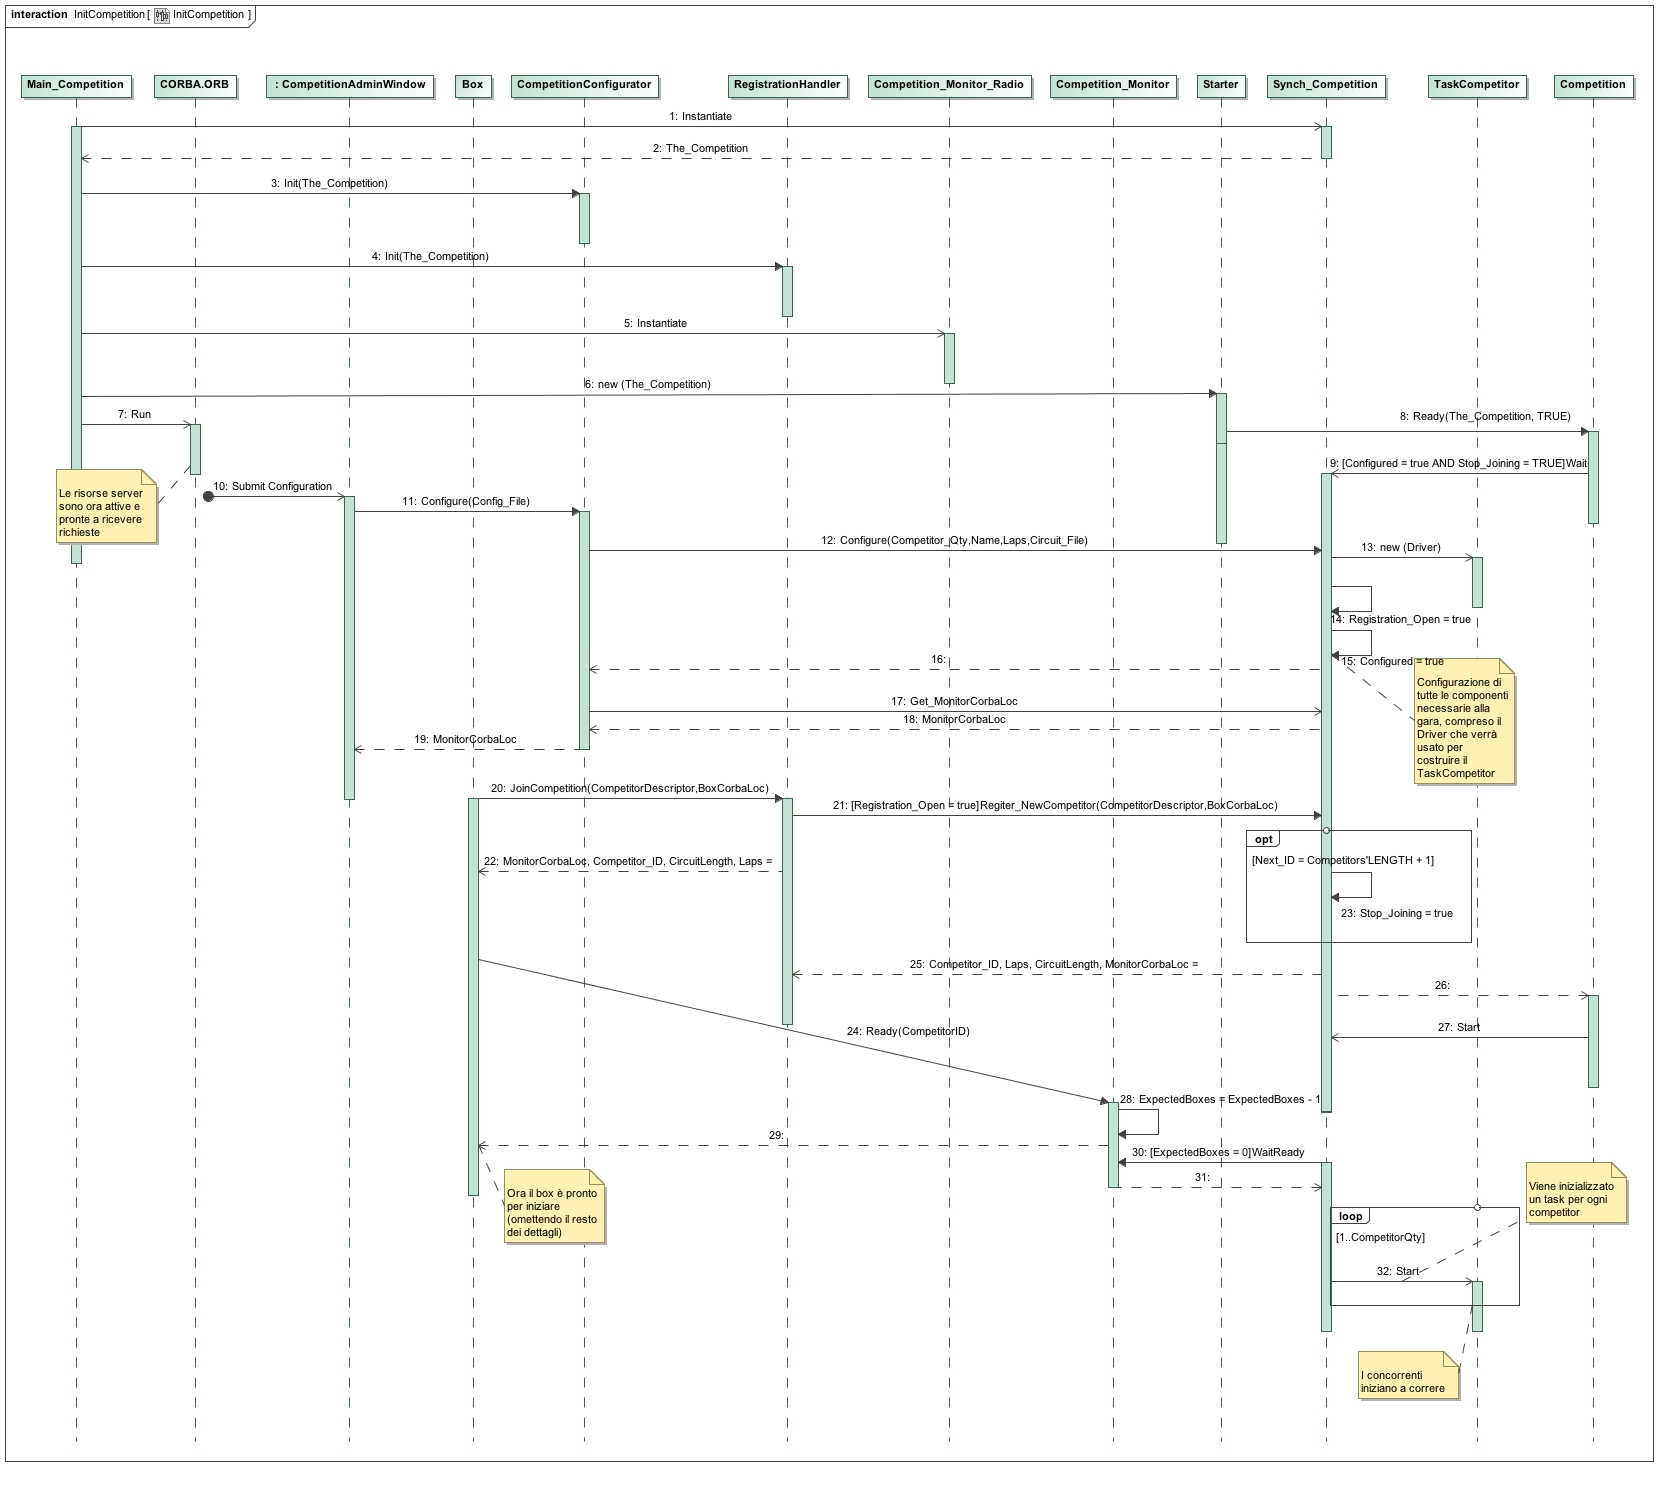
\includegraphics[angle=90,scale=0.35]{img/SequenceDiagrams/InitCompetition.jpg}
\caption{Sequence Diagram - Inizializzazione competizione}
\end{figure}
\end{center}
\clearpage
Una volta avviato il main della competizione, per prima cosa vengono
inizializzati tutti i server, vale a dire \textbf{CompetitionConfigurator},
\textbf{RegistrationHandler} e \textbf{Competition\_Monitor\_Radio}. Viene avviato
un task \textbf{Starter} che rimane in attesa
della configurazione e registrazione concorrenti avvenuti per dare lo
\underline{Start} alla gara. Viene inoltre allocata una risorsa protetta di tipo
\textbf{Synch\_Competition} pensata
per agevolare la fase di init. Ne viene condivisa un'istanza fra
\textbf{CompetitionConfigurator}, \textbf{RegistrationHandler} e
\textbf{Starter}.
Tale risorsa permette di regolare i vari step dell'inizializzazione. Finch\`{e}
la competizione non viene configurata (dal passo \textbf{10} al passo
\textbf{16}),
non sar\`{a} concesso di registrare concorrenti. Una volta configurata la
competizione, viene aperta la guardia \textsc{Registration\_Open} e il metodo
\underline{Register\_NewCompetitor} potr\`{a} essere invocato (in
\textbf{Synch\_Competition}). L'iscrizione dei concorrenti avviene a partire dai
\emph{Box}.
Nel diagramma l'azione iniziale del \emph{Box} è la \textbf{20}. In realt\`{a},
nel nodo del box, viene prima avviato uno script che esegue il main del box
seguito dal main dell'interfaccia (java) di configurazione del concorrente e del
box. A configurazione avvenuta, i parametri vengono inviati al server della
competizione invocando il metodo del server \textbf{Registration\_Handler}
\underline{Join\_Competition}, come scritto nel diagramma. A iscrizione
avvenuta, 
i parametri di configurazione della competizione tornati vengono usati per
inizializzare e avviare il box e relativi task grazie a cui successivamente
sar\`{a} possibile mandare il messaggio di \underline{Ready} alla competizione.
Quando tutti i concorrenti sono stati registrati (\textbf{23}), bisogna rimanere
in attesa della conferma di avvenuta inizializzazione dei \emph{Box}. Ci\`{o}
avviene quando il thread del task \textbf{Starter} invoca il metodo
\underline{Start} del \textbf{Synch\_Competition}, dentro cui viene messo in
attesa
sul \textbf{Competition\_Monitor} tramite \underline{Wait\_Ready}. Quando tutti
i \emph{Box} hanno dato l'ok, significa che sono pronti per ricevere
richieste dai rispettivi competitor e la gara pu\`{o} cominciare. Vengono
cos\`{i} avviati uno ad uno (\textbf{32}) e la competizione ha inizio.
\subsection{Stop competizione}
Lo stop del sistema avviene su 3 livelli: stop dei task, stop delle interfacce
utente e stop dei server. Vediamo in dettaglio:
\begin{description}
\item{\textbf{Stop dei task}}:\\
i task che devono essere fermati sono i \textbf{TaskCompetitor} lato
competizione e i task \textbf{Update\_Retriever} e \textbf{Strategy\_Updater}
lato box.
I primi si fermano in automatico quando le condizioni dell'auto non permettono
di procedere (benzina finita o gomme troppo usurate) oppure a competizione
finita
(fine ultima lap). I secondi due si fermano quando l'aggiornamento fornito dal
monitor della competizione segnala uno stato dell'auto a causa di cui il 
concorrente non pu\`{o} procedere (poca benzina o molta usura gomme), oppure
quando il concorrente finisce l'ultima lap (sempre grazie agli aggiornamenti);
\item{\textbf{Stop delle interfacce utente}}:\\
\`{e} sufficiente chiudere le interfacce con il tasto \textbf{x} in alto a
destra;
\item{\textbf{Stop dei server}}:\\
una volta finita la gara e chiuse le interfacce utente, lo script di avvio
procede l'esecuzione invocando un \textbf{killall -9} sui main avviati,
interrompendo
cos\`{i} anche i task server.
\end{description}